
\documentclass{article}
\usepackage[utf8]{inputenc}
\usepackage[english]{babel}
\usepackage[]{amsthm}
\usepackage[]{amssymb}
\usepackage[]{amsmath}
\usepackage[]{hyperref}
\usepackage[]{cancel}
\usepackage[]{graphicx}
\usepackage[]{xcolor}
\usepackage[]{tabularx}
\usepackage[]{fancyhdr}
\hypersetup{
    colorlinks,
    linkcolor={red!50!black},
    citecolor={blue!50!black},
    urlcolor={blue!80!black}
}

\pagestyle{fancy}
\fancyhf{}
\title{\vspace{-4cm}MTH30002 - Differential Equations \\Assignment 7}
\author{Joshua Rogers}
\lhead{MTH30002 Assignment 7}
\rhead{Joshua Rogers 101096819}
\date\today

\begin{document}
\maketitle

\section*{Problem 3.8}

Develop a Fourier-Legendre series for

\begin{equation}\label{38A}
f(x) = x^3-x^2+x-1
\end{equation}


\subsection*{Answer}
$$ \sum_{n=0}^{\infty} a_n P_n (x) $$
$$ a_n = \frac{2n+1}{2} \int_{-1}^{1} f(x) P_n(x) dx $$

\begin{tabular}{
  |p{\dimexpr.1\linewidth-2\tabcolsep-1.3333\arrayrulewidth}
  |p{\dimexpr.20\linewidth-2\tabcolsep-1.3333\arrayrulewidth}
  |p{\dimexpr.90\linewidth-2\tabcolsep-1.3333\arrayrulewidth}
  |p{\dimexpr.1\linewidth-2\tabcolsep-1.3333\arrayrulewidth}|
  }
  \hline
  \centering $n$     & \centering $P_n$     & \centering integral & \centering\arraybackslash $a_n$     \\ \hline
  $0$ & $1$ & $\frac{1}{2} \int_{-1}^{1} \left(x^3-x^2+x-1\right) dx$ & $\frac{-4}{3}$ \\ \hline
  $1$ & $x$ & $\frac{3}{2} \int_{-1}^{1} \left(x^4-x^3+x^2-x\right) dx$ & $\frac{8}{5}$ \\ \hline
  $2$ & $\frac{1}{2} \left(3x^2-1\right)$ & $\frac{5}{2} \cdot \frac{1}{2} \int_{-1}^{1} \left(x^3-x^2+x-1\right)\left(3x^2-1\right) dx$ & $\frac{-2}{3}$ \\ \hline
  $3$ & $\frac{1}{2} \left(5x^3-3x\right)$ & $\frac{7}{2} \cdot \frac{1}{2} \int_{-1}^{1} \left(x^3-x^2+x-1\right)\left(5x^3-3x\right) dx$ & $\frac{2}{5}$ \\ \hline
\end{tabular}


For higher powers of $n$, the coefficients are 0.

Thus,

$$
f(x) = -\frac{4}{3} P_0(x) + \frac{8}{5} P_1(x) - \frac{2}{3} P_2(x) + \frac{2}{5} P_3(x)
$$

\section*{Problem 3.9}

Develop a Fourier-Legendre series for

\begin{equation}\label{39A}
f(x) = sin(2\pi x)
\end{equation}
\subsection*{Answer}
$$ \sum_{n=0}^{\infty} a_n P_n (x) $$
$$ a_n = \frac{2n+1}{2} \int_{-1}^{1} f(x) P_n(x) dx $$

\begin{align*}
&a_0 = \frac{1}{2} \int_{-1}^{1} sin(2\pi x) P_0 dx = 0 \\
&a_1 = \frac{3}{2} \int_{-1}^{1} sin(2\pi x) P_1 dx = \frac{-3}{2\pi} \\
&a_2 = \frac{5}{2} \int_{-1}^{1} sin(2\pi x) P_2 dx = 0\\
&a_3 = \frac{7}{2} \int_{-1}^{1} sin(2\pi x) P_3 dx = \frac{7(15-4\pi^2)}{8\pi^3} \\
&a_4 = 0\\
&a_5 = \frac{-11(16\pi^4-420\pi^2+945)}{32\pi^5}\\
&a_6 = 0\\
&a_7 = \frac{-11(64\pi^6-6048\pi^4+69300\pi^2-135135)}{128\pi^7}\\
&a_8 = 0\\
&a_9 = \frac{-11(256\pi^8-63360\pi^6+2162160\pi^4-18918900\pi^2+34459425)}{512\pi^9}
\end{align*}

$M=9$ gives a pretty good approximation (higher values don't change much.)

Due to lack of space I will not write explicitly $f(x)$, but we have:
$$ f(x) \approx a_1 P_1 + a_3 P_3 + a_5 P_5 + a_7  P_7 + a_9 P_9 $$

On a common axis, for $M = [1,9]$
\begin{figure}
\centering
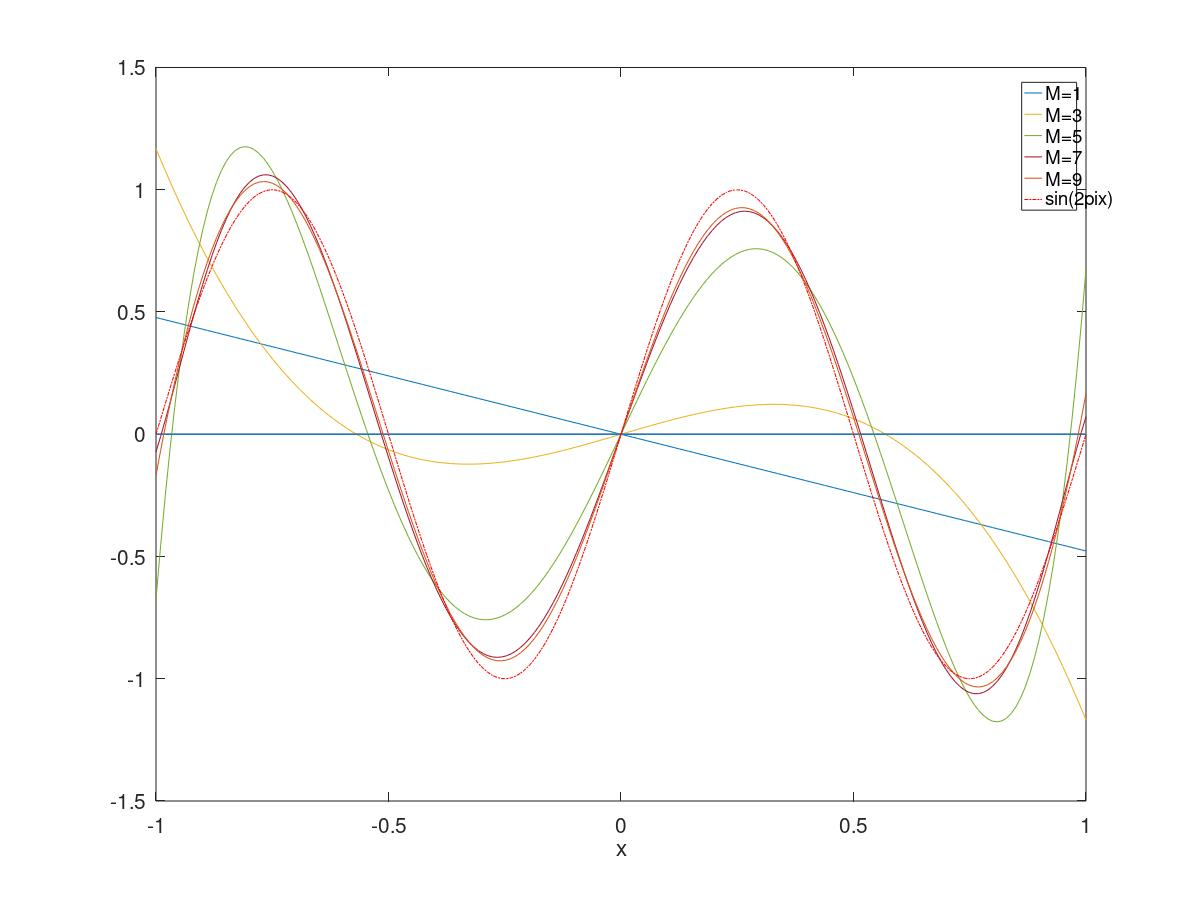
\includegraphics[width=1.0\textwidth]{./static/out.jpg}
\caption{Approximation of sums up to M=9}
\end{figure}

\pagebreak
\section*{Problem 4.1}

Find the following solutions to the following PDEs by treating them as ODEs.

\begin{align}
&u_{yy}=0 \label{41a} \\
&u_{xy}=u_x \label{41b}
\end{align}

\subsection*{Answers}

\subsubsection*{4.1 A}

For $\eqref{41a}$ we let
\begin{align*}
&u_{yy}=0 \\
&U^{''} = 0\\
\int &U^{''} = \int 0 dy \\
&U^{'} = C_1 \\
\int &U^{'} dy = \int C_1 dy \\
&U(y) = C_1y + C_2
\end{align*}

We allow $C_1 = f(x)$ and $C_2 = g(x)$, and thus obtain the solution

$$ u(x,y) = f(x)y + g(x) $$

\subsubsection*{4.2 B}

For $\eqref{41b}$ we let $u_x = V$, thus we have $V_y = V$.

We allow
\begin{align*}
\int &V^{'} dy = \int V dy \\
&V\left(y\right) = C_1 e^{y} \\
&V\left(x,y\right) = f(x) e^{y}
\end{align*}

Thus we obtain

\begin{align*}
&U_x = f(x) e^{y} \\
\int &U^{'} dx = \int f(x) e^{y} \\
&U = F\left(x\right) e^{y} + g\left(y\right)\Bigr| F\left(x\right) = \int f\left(x\right) dx
\end{align*}

Thus, we have
$$u(x,y) = e^{y} \cdot F(x) + g(y)$$


\section*{Problem 4.2}

Solve the following systems of PDEs:
\begin{align*} u_{xx} = 0 && u_{xy} =0 \end{align*}

\subsection*{Answer}

\begin{align*}
U_{xx} = 0 && u_{xy}=0\\
u_x = b(y) && u_{y} = c(y)\\
u(x,y) = b(y)x + a(y) && u(x,y) = C(y) + d(x)\Bigr|C(y) = \int c(y) dy
\end{align*}

Thus, we have the solution

$$u(x,y) = a(y) + cx$$
\end{document}
